% Standalone TikZ figure: Detection Accuracy vs Byzantine Ratio Across Datasets
% Shows PoGQ performance: MNIST (success), FEMNIST (degrades >30%), CIFAR-10 (fails)
% Compile with: pdflatex fig_detection_vs_bft.tex
\documentclass[border=5pt]{standalone}
\usepackage{pgfplots}
\pgfplotsset{compat=1.18}
\usepackage{xcolor}

\definecolor{mnistblue}{RGB}{31,119,180}
\definecolor{femnistgreen}{RGB}{44,160,44}
\definecolor{cifarred}{RGB}{214,39,40}
\definecolor{fltrustorange}{RGB}{255,127,14}

\begin{document}
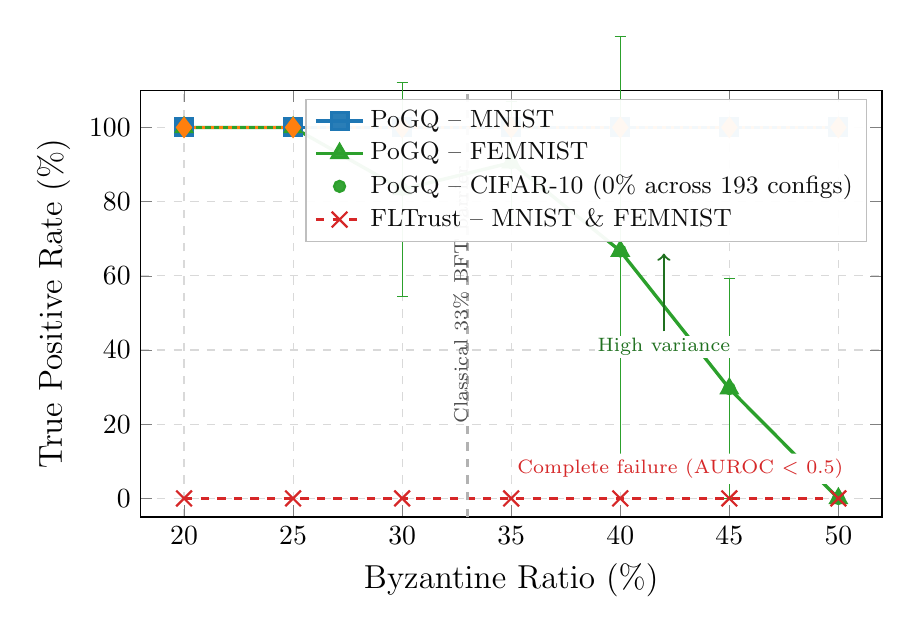
\begin{tikzpicture}
\begin{axis}[
    width=11cm,
    height=7cm,
    xlabel={Byzantine Ratio (\%)},
    ylabel={True Positive Rate (\%)},
    xlabel style={font=\large},
    ylabel style={font=\large},
    xmin=18, xmax=52,
    ymin=-5, ymax=110,
    xtick={20,25,30,35,40,45,50},
    ytick={0,20,40,60,80,100},
    grid=both,
    grid style={dashed, gray!30},
    legend style={
        at={(0.98,0.98)},
        anchor=north east,
        font=\small,
        draw=gray!50,
        fill=white,
        fill opacity=0.95,
    },
    legend cell align=left,
    clip=false,
]

% PoGQ on MNIST: 100% at all ratios
\addplot[mnistblue, very thick, mark=square*, mark size=3pt, mark options={fill=mnistblue}] coordinates {
    (20, 100) (25, 100) (30, 100) (35, 100) (40, 100) (45, 100) (50, 100)
};
\addlegendentry{PoGQ -- MNIST}

% PoGQ on FEMNIST: degrades above 30%
\addplot[femnistgreen, very thick, mark=triangle*, mark size=3pt, mark options={fill=femnistgreen}] coordinates {
    (20, 100) (25, 100) (30, 83.3) (35, 90.5) (40, 66.7) (45, 29.6) (50, 0)
};
\addlegendentry{PoGQ -- FEMNIST}

% Error bars for FEMNIST (std dev)
\addplot[femnistgreen, thick, only marks, mark=none, error bars/.cd, y dir=both, y explicit]
coordinates {
    (20, 100) +- (0, 0)
    (25, 100) +- (0, 0)
    (30, 83.3) +- (0, 28.9)
    (35, 90.5) +- (0, 16.5)
    (40, 66.7) +- (0, 57.7)
    (45, 29.6) +- (0, 29.6)
    (50, 0) +- (0, 0)
};

% PoGQ on CIFAR-10: 0% everywhere
\addplot[cifarred, very thick, dashed, mark=x, mark size=4pt, mark options={solid, cifarred, thick}] coordinates {
    (20, 0) (25, 0) (30, 0) (35, 0) (40, 0) (45, 0) (50, 0)
};
\addlegendentry{PoGQ -- CIFAR-10 (0\% across 193 configs)}

% FLTrust on FEMNIST: 100% at all ratios
\addplot[fltrustorange, very thick, dotted, mark=diamond*, mark size=3pt, mark options={fill=fltrustorange, solid}] coordinates {
    (20, 100) (25, 100) (30, 100) (35, 100) (40, 100) (45, 100) (50, 100)
};
\addlegendentry{FLTrust -- MNIST \& FEMNIST}

% Annotations
% 33% classical barrier
\draw[gray!60, thick, dashed] (axis cs:33, -5) -- (axis cs:33, 110);
\node[font=\scriptsize, gray!60!black, rotate=90, anchor=south] at (axis cs:33.5, 55) {Classical 33\% BFT barrier};

% Annotation for CIFAR-10 failure
\node[font=\scriptsize, cifarred, fill=white, inner sep=2pt, rounded corners=1pt, anchor=west]
    at (axis cs:35, 8) {Complete failure (AUROC $<$ 0.5)};

% Annotation for FEMNIST degradation
\draw[->, femnistgreen!70!black, thick] (axis cs:42, 45) -- (axis cs:42, 66);
\node[font=\scriptsize, femnistgreen!70!black, fill=white, inner sep=1pt, anchor=north] at (axis cs:42, 44) {High variance};

\end{axis}
\end{tikzpicture}
\end{document}
